\documentclass{scrartcl}
        \usepackage{xcolor, tikz}
        \usepackage{pgfplots}
        \pgfplotsset{compat=newest}
        \pagestyle{empty}
        \definecolor{pdg2112}{RGB}{228,26,28}
\definecolor{pdg2212}{RGB}{55,126,184}
\definecolor{pdg1000010020}{RGB}{153,153,153}
\definecolor{pdg1000020040}{RGB}{166,86,40}
\definecolor{pdg11}{RGB}{152,78,163}
\definecolor{pdg12}{RGB}{255,127,0}
\definecolor{pdg1000010030}{RGB}{153,153,153}
\definecolor{pdg1000050110}{RGB}{153,153,153}
\begin{document}
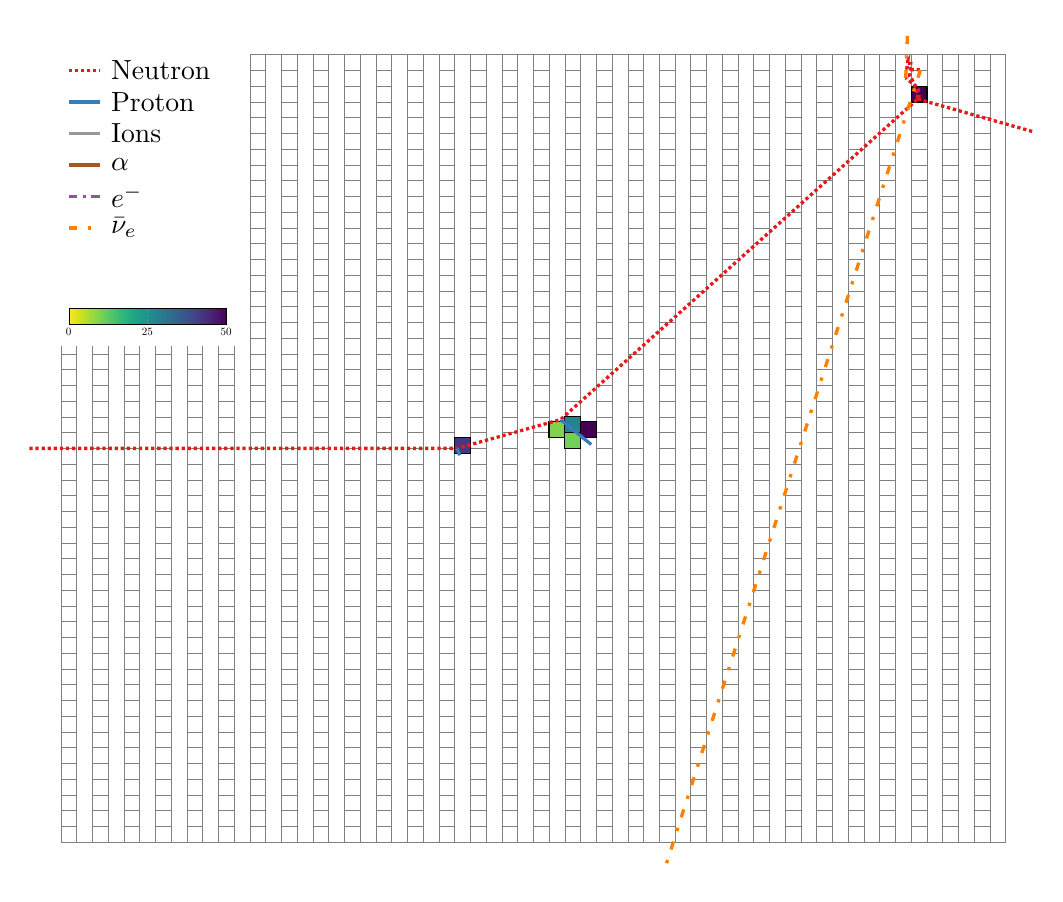
\begin{tikzpicture}[scale=0.4] %\columnwidth/252.0pt]
\draw[step=0.5,very thin,gray] (-0.001000,-12.499) grid (0.500000,3.25);
\draw[step=0.5,very thin,gray] (0.999000,-12.499) grid (1.500000,3.25);
\draw[step=0.5,very thin,gray] (1.999000,-12.499) grid (2.500000,3.25);
\draw[step=0.5,very thin,gray] (2.999000,-12.499) grid (3.500000,3.25);
\draw[step=0.5,very thin,gray] (3.999000,-12.499) grid (4.500000,3.25);
\draw[step=0.5,very thin,gray] (4.999000,-12.499) grid (5.500000,3.25);
\draw[step=0.5,very thin,gray] (5.999000,-12.499) grid (6.500000,12.499);
\draw[step=0.5,very thin,gray] (6.999000,-12.499) grid (7.500000,12.499);
\draw[step=0.5,very thin,gray] (7.999000,-12.499) grid (8.500000,12.499);
\draw[step=0.5,very thin,gray] (8.999000,-12.499) grid (9.500000,12.499);
\draw[step=0.5,very thin,gray] (9.999000,-12.499) grid (10.500000,12.499);
\draw[step=0.5,very thin,gray] (10.999000,-12.499) grid (11.500000,12.499);
\draw[step=0.5,very thin,gray] (11.999000,-12.499) grid (12.500000,12.499);
\draw[step=0.5,very thin,gray] (12.999000,-12.499) grid (13.500000,12.499);
\draw[step=0.5,very thin,gray] (13.999000,-12.499) grid (14.500000,12.499);
\draw[step=0.5,very thin,gray] (14.999000,-12.499) grid (15.500000,12.499);
\draw[step=0.5,very thin,gray] (15.999000,-12.499) grid (16.500000,12.499);
\draw[step=0.5,very thin,gray] (16.999000,-12.499) grid (17.500000,12.499);
\draw[step=0.5,very thin,gray] (17.999000,-12.499) grid (18.500000,12.499);
\draw[step=0.5,very thin,gray] (18.999000,-12.499) grid (19.500000,12.499);
\draw[step=0.5,very thin,gray] (19.999000,-12.499) grid (20.500000,12.499);
\draw[step=0.5,very thin,gray] (20.999000,-12.499) grid (21.500000,12.499);
\draw[step=0.5,very thin,gray] (21.999000,-12.499) grid (22.500000,12.499);
\draw[step=0.5,very thin,gray] (22.999000,-12.499) grid (23.500000,12.499);
\draw[step=0.5,very thin,gray] (23.999000,-12.499) grid (24.500000,12.499);
\draw[step=0.5,very thin,gray] (24.999000,-12.499) grid (25.500000,12.499);
\draw[step=0.5,very thin,gray] (25.999000,-12.499) grid (26.500000,12.499);
\draw[step=0.5,very thin,gray] (26.999000,-12.499) grid (27.500000,12.499);
\draw[step=0.5,very thin,gray] (27.999000,-12.499) grid (28.500000,12.499);
\draw[step=0.5,very thin,gray] (28.999000,-12.499) grid (29.500000,12.499);
\draw[very thin,gray] (0,-12.5) -- (30,-12.5) -- (30,12.5) -- (6,12.5);
\definecolor{tempcolor}{rgb}{0.269308,0.218818,0.509577}\draw[fill=tempcolor,fill opacity=1] (12.500000,-0.159096) rectangle (13.000000,0.340904);
\definecolor{tempcolor}{rgb}{0.506271,0.828786,0.300362}\draw[fill=tempcolor,fill opacity=1] (15.500000,0.345354) rectangle (16.000000,0.845354);
\definecolor{tempcolor}{rgb}{0.449368,0.813768,0.335384}\draw[fill=tempcolor,fill opacity=1] (16.000000,0.000000) rectangle (16.500000,0.500000);
\definecolor{tempcolor}{rgb}{0.149039,0.508051,0.557250}\draw[fill=tempcolor,fill opacity=1] (16.000000,0.500000) rectangle (16.500000,1.000000);
\definecolor{tempcolor}{rgb}{0.267004,0.004874,0.329415}\draw[fill=tempcolor,fill opacity=1] (16.500000,0.343874) rectangle (17.000000,0.843874);
\definecolor{tempcolor}{rgb}{0.267004,0.004874,0.329415}\draw[fill=tempcolor,fill opacity=1] (27.000000,11.000000) rectangle (27.500000,11.500000);
\draw[color=pdg2112, very thick, densely dotted] (-1.0007236377721482, 0.0010262730845484664) -- (-0.0007284944014827488, 0.0010331608233709393) -- (0.5029999999999746, 0.0010366303905282159) -- (0.9899999999999863, 0.0010399847356255712) -- (1.5029999999999972, 0.001043518162802046) -- (1.9899999999999864, 0.001046872507899401) -- (2.5029999999999974, 0.0010504059350758758) -- (2.9899999999999864, 0.001053760280173231) -- (3.5029999999999974, 0.0010572937073497057) -- (3.9899999999999864, 0.0010606480524470608) -- (4.5029999999999974, 0.0010641814796235355) -- (4.989999999999986, 0.0010675358247208906) -- (5.5029999999999974, 0.0010710692518973654) -- (5.989999999999986, 0.0010744235969947205) -- (6.5029999999999974, 0.0010779570241711953) -- (6.989999999999986, 0.0010813113692685506) -- (7.5029999999999974, 0.0010848447964450253) -- (7.863636909912043, 0.001087328781354037) -- (7.9970000000000026, 0.0010882473559482972) -- (8.502999999999975, 0.0010917325687188552) -- (8.997000000000003, 0.0010951351282221273) -- (9.996995143370645, 0.0011020228670446) -- (10.996990286741312, 0.001108910605867073) -- (11.502999999999975, 0.0011123958855403448) -- (11.997000000000003, 0.0011157984450436169) -- (12.502999999999975, 0.0011192836578141747) -- (12.58157564356934, 0.00111982486895335) -- (12.643032382206366, 0.018220210203299884) -- (12.742584515139379, 0.045920668635777706) -- (12.825544625916882, 0.06900438399617488) -- (12.85872867022788, 0.07823787014033408) -- (12.989999999999986, 0.11476421976838327) -- (13.489999999999986, 0.2538896087297683) -- (13.990000000000009, 0.39301499769115333) -- (14.33855249294495, 0.49000000000000005) -- (14.363709655315734, 0.497) -- (14.38527293734785, 0.5030000000000001) -- (14.403242339041253, 0.5079999999999999) -- (14.489999999999963, 0.5321403866525276) -- (14.990000000000009, 0.6712657756139127) -- (15.490000000000009, 0.810391164575285) -- (15.868600930658113, 0.9157371680531773) -- (15.990000000000009, 1.0247292191512358) -- (16.49000000000001, 1.473629081765147) -- (16.99000000000001, 1.9225289443790583) -- (17.06515156635164, 1.9899999999999998) -- (17.49000000000001, 2.371428806992972) -- (17.99000000000001, 2.8203286696068828) -- (18.178985723235837, 2.99) -- (18.49000000000001, 3.2692285322208017) -- (18.99000000000001, 3.718128394834713) -- (19.29281988012001, 3.9900000000000007) -- (19.489999999999963, 4.167028257448632) -- (19.99000000000001, 4.615928120062523) -- (20.406654037004227, 4.99) -- (20.49000000000001, 5.064827982676443) -- (20.99000000000001, 5.5137278452903535) -- (21.49000000000001, 5.962627707904264) -- (21.99000000000001, 6.411527570518176) -- (22.07740527233052, 6.49) -- (22.49000000000001, 6.860427433132111) -- (22.99000000000001, 7.309327295746021) -- (23.191239429214694, 7.489999999999999) -- (23.49000000000001, 7.758227158359942) -- (23.99000000000001, 8.207127020973854) -- (24.30507358609889, 8.489999999999998) -- (24.49000000000001, 8.656026883587794) -- (24.99000000000001, 9.104926746201704) -- (25.418907742983084, 9.49) -- (25.49000000000001, 9.553826608815623) -- (25.99000000000001, 10.002726471429533) -- (26.49000000000001, 10.451626334043445) -- (26.99000000000001, 10.900526196657355) -- (27.08965897830935, 10.99) -- (27.20351712212814, 11.092221810235461);
\draw[color=pdg1000020040, very thick, solid] (27.20351712212814, 11.092221810235461);
\draw[color=pdg2212, very thick, solid] (27.20351712212814, 11.092221810235461) -- (27.20386765888304, 11.122943084519267) -- (27.204051628458593, 11.147648428517261) -- (27.20448330978461, 11.16790984550521) -- (27.20494185745026, 11.183989480900788) -- (27.205442676520192, 11.19685047504636) -- (27.20598114076902, 11.207296452954669) -- (27.206208818604956, 11.215521235369787) -- (27.20656261370459, 11.221976068468184);
\draw[color=pdg2212, very thick, solid] (27.20351712212814, 11.092221810235461);
\draw[color=pdg1000010020, very thick, solid] (27.20351712212814, 11.092221810235461) -- (27.226803917168855, 11.114584568018868) -- (27.2352483479548, 11.123153225390512);
\draw[color=pdg1000050110, very thick, solid] (27.2352483479548, 11.123153225390512);
\draw[color=pdg2212, very thick, solid] (27.2352483479548, 11.123153225390512);
\draw[color=pdg2212, very thick, solid] (27.2352483479548, 11.123153225390512) -- (27.244146467094698, 11.12347064789258);
\draw[color=pdg2112, very thick, densely dotted] (27.2352483479548, 11.123153225390512) -- (27.250017836540973, 11.209044740636767) -- (27.21950269658837, 11.413828338833843) -- (27.185756939982003, 11.46192376619656) -- (27.152011102970437, 11.49) -- (27.14359755075632, 11.497000000000002) -- (27.136385934572807, 11.503) -- (27.130376254419865, 11.508) -- (27.00999999999997, 11.60815196429468) -- (26.99699999999998, 11.618967847727033) -- (26.957809750565115, 11.651573783848026) -- (26.824992403187753, 11.762076625927302);
\draw[color=pdg11, very thick, dashdotted] (26.824992403187753, 11.762076625927302);
\draw[color=pdg12, very thick, loosely dashdotted] (26.824992403187753, 11.762076625927302) -- (26.852963699867587, 12.4666066117045) -- (26.85338531698494, 12.477226137323893) -- (26.854439359778347, 12.503774951372375) -- (26.855704211130433, 12.535633528230557) -- (26.85675825392384, 12.562182342279039) -- (26.857179871041193, 12.57280186789843) -- (26.88402723530471, 13.249022687377325) -- (26.88469734172504, 13.265901063527926) -- (26.886278441757987, 13.305725187395641);
\draw[color=pdg2212, very thick, solid] (26.824992403187753, 11.762076625927302);
\draw[color=pdg2212, very thick, solid] (26.824992403187753, 11.762076625927302);
\draw[color=pdg1000010030, very thick, solid] (27.20351712212814, 11.092221810235461);
\draw[color=pdg2112, very thick, densely dotted] (27.20351712212814, 11.092221810235461) -- (27.156208569854336, 11.457099052559823) -- (27.139675571192424, 11.489999999999998) -- (27.014535047647133, 11.739031761993054) -- (27.010000000000012, 11.744095764845872) -- (27.002999999999997, 11.751912225162915) -- (26.997000000000025, 11.758612048291804) -- (26.952222583259733, 11.811790669725628) -- (26.985117259883918, 12.217923544323588) -- (26.917459642922562, 12.22587930374178) -- (26.85648325094892, 12.255064867913791) -- (26.890322674826827, 12.305709200327282) -- (26.86200428930356, 12.07456534549695) -- (26.968711638435686, 12.030224408488163) -- (26.99000000000001, 12.02551519795044) -- (27.0363731667323, 12.021216594936494) -- (27.293150092686027, 12.021478660436431);
\draw[color=pdg11, very thick, dashdotted] (27.293150092686027, 12.021478660436431);
\draw[color=pdg12, very thick, loosely dashdotted] (27.293150092686027, 12.021478660436431) -- (27.289476835542974, 12.010000000000002) -- (27.12947309802439, 11.510000000000002) -- (27.010000000000012, 11.136655289816208) -- (27.002999999999997, 11.114780800793163) -- (26.997000000000025, 11.096031238773422) -- (26.991999999999983, 11.080406603756888) -- (26.510000000000012, 9.574191788168674) -- (26.502999999999997, 9.552317299145631) -- (26.497000000000025, 9.533567737125889) -- (26.491999999999983, 9.517943102109356) -- (26.329454410431435, 9.010000000000002) -- (26.169450672912877, 8.510000000000002) -- (26.010000000000012, 8.011728286520995) -- (25.997000000000025, 7.971104235478231) -- (25.991999999999983, 7.955479600461696) -- (25.88327716108613, 7.615728665264896) -- (25.874771213238386, 7.589148199146889) -- (25.853506343619053, 7.522697033851898) -- (25.827988500075843, 7.442955635497894) -- (25.80672363045651, 7.376504470202901) -- (25.798217682608787, 7.349924004084903) -- (25.510000000000012, 6.449264784873565) -- (25.502999999999997, 6.427390295850522) -- (25.497000000000025, 6.408640733830781) -- (25.491999999999983, 6.393016098814246) -- (25.369431985319828, 6.01) -- (25.20942824780127, 5.51) -- (25.049424510282712, 5.01) -- (25.010000000000012, 4.886801283225898) -- (25.002999999999997, 4.864926794202853) -- (24.997000000000025, 4.846177232183112) -- (24.991999999999983, 4.830552597166578) -- (24.510000000000012, 3.3243377815783655) -- (24.502999999999997, 3.3024632925553212) -- (24.497000000000025, 3.28371373053558) -- (24.491999999999983, 3.268089095519046) -- (24.409409560208314, 3.0100000000000002) -- (24.24940582268973, 2.51) -- (24.089402085171173, 2.0100000000000002) -- (24.010000000000012, 1.7618742799306155) -- (24.002999999999997, 1.739999790907572) -- (23.997000000000025, 1.7212502288878304) -- (23.991999999999983, 1.705625593871296) -- (23.75679019915308, 0.9706121357651807) -- (23.748284251305357, 0.9440316696471888) -- (23.727019381686024, 0.8775805043521837) -- (23.701501538142814, 0.7978391059981844) -- (23.68023666852348, 0.7313879407031877) -- (23.671730720675736, 0.7048074745851952) -- (23.510000000000012, 0.19941077828321696) -- (23.502999999999997, 0.17753628926017334) -- (23.497000000000025, 0.15878672724043197) -- (23.491999999999983, 0.14316209222389767) -- (23.449387135096732, 0.01) -- (23.28938339757817, -0.48999999999999994) -- (23.129379660059612, -0.9899999999999999) -- (23.010000000000012, -1.363052723364524) -- (23.002999999999997, -1.3849272123875678) -- (22.997000000000025, -1.4036767744073089) -- (22.991999999999983, -1.4193014094238434) -- (22.510000000000012, -2.9255162250120557) -- (22.502999999999997, -2.947390714035099) -- (22.497000000000025, -2.966140276054841) -- (22.491999999999983, -2.9817649110713753) -- (22.32936097246668, -3.4899999999999998) -- (22.16935723494812, -3.9900000000000007) -- (22.010000000000012, -4.487979726659876) -- (21.997000000000025, -4.528603777702713) -- (21.991999999999983, -4.544228412719248) -- (21.63030323722012, -5.674504393734518) -- (21.621797289372374, -5.701084859852523) -- (21.60053241975304, -5.767536025147523) -- (21.57501457620983, -5.847277423501517) -- (21.553749706590498, -5.913728588796518) -- (21.545243758742778, -5.940309054914524) -- (21.510000000000012, -6.050443228307426) -- (21.502999999999997, -6.072317717330469) -- (21.497000000000025, -6.09106727935021) -- (21.491999999999983, -6.106691914366744) -- (21.369338547355163, -6.49) -- (21.209334809836584, -6.989999999999999) -- (21.049331072318022, -7.489999999999999) -- (21.010000000000012, -7.612906729955188) -- (21.002999999999997, -7.634781218978231) -- (20.997000000000025, -7.653530780997973) -- (20.991999999999983, -7.669155416014506) -- (20.510000000000012, -9.17537023160272) -- (20.502999999999997, -9.197244720625765) -- (20.497000000000025, -9.215994282645505) -- (20.491999999999983, -9.231618917662038) -- (20.409316122243627, -9.49) -- (20.249312384725066, -9.989999999999998) -- (20.089308647206508, -10.49) -- (20.010000000000012, -10.737833733250397) -- (20.002999999999997, -10.759708222273442) -- (19.997000000000025, -10.778457784293183) -- (19.991999999999983, -10.794082419309717) -- (19.510000000000012, -12.30029723489793) -- (19.502999999999997, -12.322171723920972) -- (19.497000000000025, -12.340921285940713) -- (19.491999999999983, -12.356545920957247) -- (19.449293697132088, -12.489999999999998) -- (19.14305108226779, -13.446985816749267);
\draw[color=pdg2212, very thick, solid] (27.293150092686027, 12.021478660436431);
\draw[color=pdg2212, very thick, solid] (26.85648325094892, 12.255064867913791);
\draw[color=pdg2212, very thick, solid] (26.917459642922562, 12.22587930374178);
\draw[color=pdg2212, very thick, solid] (26.952222583259733, 11.811790669725628);
\draw[color=pdg2212, very thick, solid] (26.99412058469047, 11.761827310506563);
\draw[color=pdg2112, very thick, densely dotted] (27.20351712212814, 11.092221810235461) -- (27.49000000000001, 11.011150860039487) -- (27.99000000000001, 10.869657325071163) -- (28.49000000000001, 10.728163790102837) -- (28.99000000000001, 10.586670255134514) -- (29.260932008136205, 10.510000000000002) -- (29.285668120643276, 10.503) -- (29.306870502792208, 10.497000000000002) -- (29.324539154582975, 10.491999999999999) -- (29.49000000000001, 10.445176720166193) -- (29.99000000000001, 10.30368318519787) -- (30.868756499429765, 10.055006458236466);
\draw[color=pdg2212, very thick, solid] (15.868600930658113, 0.9157371680531773) -- (15.990000000000009, 0.8163783880867822) -- (16.1801442522019, 0.6585800214755131) -- (16.31644198553438, 0.5478805756216282) -- (16.362397645301552, 0.51) -- (16.484103841972182, 0.41166842638813456) -- (16.586459129093054, 0.3275608127949255) -- (16.64323609369376, 0.28160449561560147) -- (16.68912708730941, 0.24456458531723696) -- (16.725998637259544, 0.21539066309005978) -- (16.755455676134922, 0.19281239285104837) -- (16.778583235096743, 0.1738764271645123) -- (16.796811762943616, 0.15875579199520334) -- (16.81127590983267, 0.14653161677740772) -- (16.82291855722274, 0.13674517078234602) -- (16.832315548642804, 0.1290295485362555) -- (16.839805542532826, 0.12286079016752219);
\draw[color=pdg2212, very thick, solid] (12.58157564356934, 0.00111982486895335) -- (12.60621961362906, -0.061454273136120195) -- (12.621069203673915, -0.1004656495841603) -- (12.632962693174296, -0.1321986204466646) -- (12.64211697051976, -0.15773005111666355) -- (12.648906206574498, -0.17831972513696456) -- (12.654351264707316, -0.19490048690611567) -- (12.658976459302085, -0.2081388046552438) -- (12.662628096753973, -0.21875652236018092);
\draw[color=pdg2112, very thick, densely dotted] (0.25,12) -- (1.25,12) node [right,black] {Neutron};
\draw[color=pdg2212, very thick, solid] (0.25,11) -- (1.25,11) node [right,black] {Proton};
\draw[color=pdg1000010020, very thick, solid] (0.25,10) -- (1.25,10) node [right,black] {Ions};
\draw[color=pdg1000020040, very thick, solid] (0.25,9) -- (1.25,9) node [right,black] {$\alpha$};
\draw[color=pdg11, very thick, dashdotted] (0.25,8) -- (1.25,8) node [right,black] {$e^-$};
\draw[color=pdg12, very thick, loosely dashdotted] (0.25,7) -- (1.25,7) node [right,black] {$\bar{\nu}_e$};

        \begin{axis}[%
            at={(0.25cm,4.75cm)},
            hide axis,
            scale only axis,
            height=0pt,
            width=0pt,
            colormap={reverse viridis}{
                indices of colormap={
                \pgfplotscolormaplastindexof{viridis},...,0 of viridis}
            },
            colorbar horizontal,
            point meta min=0,
            point meta max=50,
            colorbar style={
                width=5cm,
                xtick={50, 25, 0},
            }]
        \end{axis}
        
        \end{tikzpicture}
        \end{document}
        